\documentclass[10pt,a4paper]{amsart}
\usepackage[margin=19mm]{geometry}
\usepackage{amsmath,amssymb,mathtools}
\usepackage[scr=rsfs,cal=euler]{mathalfa}
\usepackage{xfrac}
\usepackage[unicode,hidelinks,bookmarks=false]{hyperref}
\newcommand{\ie}{i.e.\ }
\newcommand{\cf}{cf.\ }
\newcommand{\resp}{respectively\ }
\newcommand{\Subsection}{\subsection}
\providecommand{\nobreakdash}{\nobreak\hbox{-}}
\setlength{\emergencystretch}{2em}
\multlinegap0pt
\usepackage{tikz}
\usetikzlibrary{cd}
\usepackage{tikz}
\usepackage{amssymb}
\usepackage[normalem]{ulem}
\usepackage{mathtools}
\newtheorem{lem}{Lemma}
\newtheorem{prop}{Proposition}
\DeclareMathOperator{\Comp}{C}
\DeclareMathOperator{\Part}{\rho}
\newcommand{\RP}{\mathbb{R}\mathrm{P}}
\newcommand{\Z}{\mathbb{Z}}
\newcommand{\allfr}{\catname{Fr}}
\newcommand{\aut}{\operatorname{aut}}
\newcommand{\catname}[1]{{\normalfont\textbf{#1}}}
\DeclareMathOperator{\ce}{cr}
\newcommand{\ch}{\catname{Ch}}
\newcommand{\classifying}{\operatorname{B}}
\newcommand{\fr}{\allfr^{\mathrm{fg}}}
\DeclareMathOperator{\hocolim}{hocolim \,}
\DeclareMathOperator{\map}{Map}
\newcommand{\mset}{\catname{MSet}}
\DeclareMathOperator{\nat}{Nat}
\DeclareMathOperator{\pointedmaps}{\map_*}
\DeclareMathOperator{\spectralNat}{\underline{\underline{\nat}}}
\title{Polynomial functors from free groups to a stable $\infty$-category}
\author{Gregory Arone}
\date{Source: arXiv:2504.04114v3 (CC BY 4.0)}
\begin{document}
\maketitle

\noindent\emph{Source and licence.} Polynomial functors from free groups to a stable $\infty$-category. Version arXiv:2504.04114v3 (CC BY 4.0), distributed by arXiv under the Creative Commons Attribution 4.0 International licence, http://creativecommons.org/licenses/by/4.0/, as recorded in the arXiv licence metadata for this exact version and shown on the abstract page https://arxiv.org/abs/2504.04114v3. Full licence notice: \texttt{licenses/arxiv-2504.04114-CC-BY-4.0.txt}.\par\smallskip

\noindent\textit{Editorial scope.} Counted unit: the article's prop sym3x (source0.tex lines 2691--2698). The article's complete original proof of it is delivered with it (source0.tex lines 2699--3004, one \texttt{proof} environment of 306 lines). No mathematics is written, repaired or re-derived: the statement and the proof are the article's own lines, in the article's own notation, and no retained line is substituted or re-flowed.  Retained uncounted as the source-local context the proof needs: lines 2564--2566; lines 2568--2570; lines 2575--2576.  Nothing was omitted from any retained span, so the package carries no omission record.  No retained line contains a citation, so the wrapper carries no bibliography and no bibliography entry.  The retained lines contain the article's own diagram code, which the wrapper typesets with the standard tikz packages; no image file is delivered and the package declares no asset dependency.  Editorial formatting only, in addition: an AMS \texttt{amsart} preamble that restates the article's own declarations and macros used by the retained lines, namely the environments \texttt{lem}, \texttt{prop} on separate counters, together with the standard packages those lines need.  The retained environments print in this document as Lemma 1, Proposition 1 in order of appearance, whereas the article prints the same items with the numbering of its own full document.  The complete native source of the article as distributed in the arXiv e-print for this exact version is bundled unchanged as \texttt{sources/176033/source0.tex}.
\begin{equation}\label{eq:cubical model}
\{i_0, \ldots, i_p\}\mapsto \underset{\underline{i_0}\leftarrow \cdots \leftarrow \underline{i_p}\in \operatorname{Iso}(i_0, \ldots, i_p)}{\hocolim} X^{\wedge i_0}.
\end{equation}

\begin{equation}\label{eq: crude cubical model}
\underset{\underline{i_0}\leftarrow \cdots \leftarrow \underline{i_p}\in\operatorname{Iso}(i_0, \ldots, i_p)}{\hocolim} X^{\wedge i_0}\simeq \bigvee_{[\underline{i_0}\leftarrow \cdots \leftarrow \underline{i_p}]} X^{\wedge i_0}_{h\aut(\underline{i_0}\leftarrow \cdots \leftarrow \underline{i_p})}.
\end{equation}

\begin{lem}\label{lem: cubical orbits}
Let $X$ be a pointed CW complex. The space $X^{\wedge n}_{\Sigma_n}$ is naturally equivalent to the homotopy colimit of the cubical diagram~\eqref{eq:cubical model} (which up to homotopy is the same as the right hand side of~\eqref{eq: crude cubical model}). \end{lem}

\begin{prop}\label{prop:nat from sym3x}
$\spectralNat_X(\widetilde \Z[(X^{\wedge 3})_{\Sigma_3}], \widetilde \Z[(X^{\wedge n})_{\Sigma_n}])$ is equivalent to
\[ \begin{array}{lc}
   \Z[\Part(n, 3)]\times \Sigma^{-1}\pointedmaps(\RP^\infty, \Z)^{\lfloor\frac{n}{2}\rfloor} & \mbox{if }3\mid n \\[10pt]
   \Z[\Part(n, 3)]\times \Sigma^{-1}\pointedmaps(\RP^\infty, \Z)^{\lfloor\frac{n}{2}\rfloor} \times \Sigma^{-1}\pointedmaps(\classifying\Sigma_3/\classifying \Sigma_2 , \Z) & \mbox{if }3\nmid n 
   \end{array}
\]
\end{prop}

\begin{proof}
We want to use the case $n=3$ of Lemma~\ref{lem: cubical orbits} to resolve $(X^{\wedge 3})_{\Sigma_3}$ as a homotopy colimit of a cubical diagram. The cube is indexed by isomorphism classes of chains in $\mset_3$. Recall that $\mset_3$ is the category of multisets of total multiplicity $3$. The following diagram indicates the isomorphism classes of chains in $\mset_3$ together with the corresponding groups of automorphisms (when the group is non-trivial).

\tikzset{every picture/.style={line width=0.75pt}} %set default line width to 0.75pt        
\[
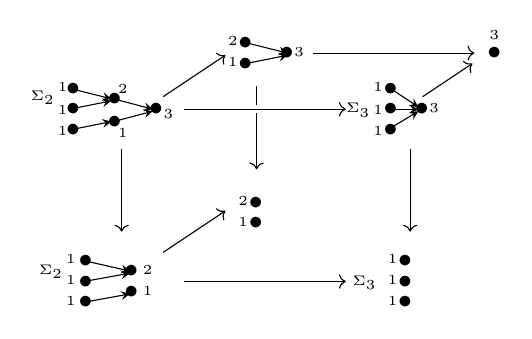
\begin{tikzpicture}[x=0.75pt,y=0.75pt,yscale=-1,xscale=1]
%uncomment if require: \path (0,300); %set diagram left start at 0, and has height of 300

%Straight Lines [id:da8478941034785542] 
\draw [-stealth]   (45,91) -- (65,96) ;

\draw  [-stealth]  (45,101) -- (65,97) ;
 
\draw   [-stealth] (45,111) -- (65,107) ;

\draw  [-stealth]  (66,96) -- (85,101) ;

\draw  [-stealth]  (66,107) -- (85,102) ;


% Text Node
\draw (42,87) node [anchor=north west][inner sep=0.75pt]    {$\bullet $};
% Text Node
\draw (42,107) node [anchor=north west][inner sep=0.75pt]    {$\bullet $};
% Text Node
\draw (42,97) node [anchor=north west][inner sep=0.75pt]    {$\bullet $};
% Text Node
\draw (62,92) node [anchor=north west][inner sep=0.75pt]    {$\bullet $};
% Text Node
\draw (62,103) node [anchor=north west][inner sep=0.75pt]    {$\bullet $};
% Text Node
\draw (82,97) node [anchor=north west][inner sep=0.75pt]    {$\bullet $};
% Text Node

\draw (25,91) node [anchor=north west][inner sep=0.75pt]  [font=\tiny] [align=left] {$\Sigma_2$};

\draw (38,87) node [anchor=north west][inner sep=0.75pt]  [font=\tiny] [align=left] {$\displaystyle 1$};
% Text Node
\draw (38,108) node [anchor=north west][inner sep=0.75pt]  [font=\tiny] [align=left] {$\displaystyle 1$};
% Text Node
\draw (38,98) node [anchor=north west][inner sep=0.75pt]  [font=\tiny] [align=left] {$\displaystyle 1$};
% Text Node
\draw (67,109) node [anchor=north west][inner sep=0.75pt]  [font=\tiny] [align=left] {$\displaystyle 1$};
% Text Node
\draw (67,88) node [anchor=north west][inner sep=0.75pt]  [font=\tiny] [align=left] {$\displaystyle 2$};
% Text Node
\draw (89,100) node [anchor=north west][inner sep=0.75pt]  [font=\tiny] [align=left] {$\displaystyle 3$};

\draw [->] (90, 95)-- (120, 75);

% Text Node
\draw (125,65) node [anchor=north west][inner sep=0.75pt]    {$\bullet $};
% Text Node
\draw (125,75) node [anchor=north west][inner sep=0.75pt]    {$\bullet $};
% Text Node
\draw (145,70) node [anchor=north west][inner sep=0.75pt]    {$\bullet $};

\draw (120,65) node [anchor=north west][inner sep=0.75pt]  [font=\tiny] [align=left] {$\displaystyle 2$};
% Text Node
\draw (120,75) node [anchor=north west][inner sep=0.75pt]  [font=\tiny] [align=left] {$\displaystyle 1$};
% Text Node
\draw (152,70) node [anchor=north west][inner sep=0.75pt]  [font=\tiny] [align=left] {$\displaystyle 3$};
\draw[-stealth] (130,69)--(150,74);
\draw[-stealth] (130,79)--(150,75);

\draw [->] (100, 101)-- (178, 101);

\draw (195,87) node [anchor=north west][inner sep=0.75pt]    {$\bullet $};
% Text Node
\draw (195,107) node [anchor=north west][inner sep=0.75pt]    {$\bullet $};
% Text Node
\draw (195,97) node [anchor=north west][inner sep=0.75pt]    {$\bullet $};

\draw (190,87) node [anchor=north west][inner sep=0.75pt]  [font=\tiny] [align=left] {$\displaystyle 1$};
% Text Node
\draw (190,108) node [anchor=north west][inner sep=0.75pt]  [font=\tiny] [align=left] {$\displaystyle 1$};
% Text Node
\draw (190,98) node [anchor=north west][inner sep=0.75pt]  [font=\tiny] [align=left] {$\displaystyle 1$};

\draw (177,97) node [anchor=north west][inner sep=0.75pt]  [font=\tiny] [align=left] {$\Sigma_3$};

\draw (217,97) node [anchor=north west][inner sep=0.75pt]  [font=\tiny] [align=left] {$3$};

\draw (210,97) node [anchor=north west][inner sep=0.75pt]    {$\bullet $};

\draw[-stealth] (198,90)--(213,100);
\draw[-stealth] (198,101)--(213,101);
\draw[-stealth] (198,111)--(213,102);

\draw[->] (162,74)--(240,74);
\draw [->] (215, 95)-- (239, 79);

\draw (245,70) node [anchor=north west][inner sep=0.75pt]    {$\bullet $};

\draw (246,62) node [anchor=north west][inner sep=0.75pt]  [font=\tiny] [align=left] {$\displaystyle 3$};

\draw [->] (70, 120)-- (70, 160);
\draw [->] (209, 120)-- (209, 160);

\draw (48,170) node [anchor=north west][inner sep=0.75pt]    {$\bullet $};
% Text Node
\draw (48,180) node [anchor=north west][inner sep=0.75pt]    {$\bullet $};
% Text Node
\draw (48,190) node [anchor=north west][inner sep=0.75pt]    {$\bullet $};
% Text Node
\draw (70,175) node [anchor=north west][inner sep=0.75pt]    {$\bullet $};
% Text Node
\draw (70,185) node [anchor=north west][inner sep=0.75pt]    {$\bullet $};
\draw[-stealth] (52, 174)--(74,179);
\draw[-stealth] (52, 184)--(74,180);
\draw[-stealth] (52, 194)--(74,190);

\draw (29,175) node [anchor=north west][inner sep=0.75pt]  [font=\tiny] [align=left] {$\Sigma_2$};

\draw (42,170) node [anchor=north west][inner sep=0.75pt]  [font=\tiny] [align=left] {$\displaystyle 1$};
% Text Node
\draw (42,180) node [anchor=north west][inner sep=0.75pt]  [font=\tiny] [align=left] {$\displaystyle 1$};
% Text Node
\draw (42,190) node [anchor=north west][inner sep=0.75pt]  [font=\tiny] [align=left] {$\displaystyle 1$};
% Text Node
\draw (79,185) node [anchor=north west][inner sep=0.75pt]  [font=\tiny] [align=left] {$\displaystyle 1$};
% Text Node
\draw (79,175) node [anchor=north west][inner sep=0.75pt]  [font=\tiny] [align=left] {$\displaystyle 2$};

\draw[->] (100,184)--(178,184);

\draw (202,170) node [anchor=north west][inner sep=0.75pt]    {$\bullet $};
% Text Node
\draw (202,180) node [anchor=north west][inner sep=0.75pt]    {$\bullet $};
% Text Node
\draw (202,190) node [anchor=north west][inner sep=0.75pt]    {$\bullet $};

\draw (197,170) node [anchor=north west][inner sep=0.75pt]  [font=\tiny] [align=left] {$\displaystyle 1$};
% Text Node
\draw (197,180) node [anchor=north west][inner sep=0.75pt]  [font=\tiny] [align=left] {$\displaystyle 1$};
% Text Node
\draw (197,190) node [anchor=north west][inner sep=0.75pt]  [font=\tiny] [align=left] {$\displaystyle 1$};

\draw (180,180) node [anchor=north west][inner sep=0.75pt]  [font=\tiny] [align=left] {$\Sigma_3$};

\draw [->] (90, 170)-- (120, 150);

\draw (125,152) node [anchor=north west][inner sep=0.75pt]  [font=\tiny] [align=left] {$\displaystyle 1$};
% Text Node
\draw (125,142) node [anchor=north west][inner sep=0.75pt]  [font=\tiny] [align=left] {$\displaystyle 2$};
\draw (130,152) node [anchor=north west][inner sep=0.75pt]    {$\bullet $};
% Text Node
\draw (130,142) node [anchor=north west][inner sep=0.75pt]    {$\bullet $};

\draw (135, 90)--(135, 99);
\draw[->](135, 103)--(135, 130);

\end{tikzpicture}
\]
Recall that the cubical diagram in Lemma~\ref{lem: cubical orbits} that resolves $(X^{\wedge n})_{\Sigma_n}$ sends a chain $\underline {i_k}\to \cdots \to \underline{i_0}$ to $X^{\wedge i_0}_{h\aut(\underline {i_k}\to \cdots \to \underline{i_0})}$. It follows that there is a homotopy pushout cubes of functors
\[\begin{tikzcd}
	& X && X \\
	{X\wedge\RP^\infty_+} & {} & {X\wedge{\classifying \Sigma_3}_+} \\
	& {X\wedge X} & {} & {X^{\wedge 3}_{\Sigma_3}} \\
	{X\wedge X\wedge \RP^\infty_+} && {X^{\wedge 3}_{h\Sigma_3}}
	\arrow[from=1-2, to=1-4]
	\arrow[no head, from=1-2, to=2-2]
	\arrow[from=1-4, to=3-4]
	\arrow[from=2-1, to=1-2]
	\arrow[from=2-1, to=2-3]
	\arrow[from=2-1, to=4-1]
	\arrow[from=2-2, to=3-2]
	\arrow[from=2-3, to=1-4]
	\arrow[from=2-3, to=4-3]
	\arrow[no head, from=3-2, to=3-3]
	\arrow[from=3-3, to=3-4]
	\arrow[from=4-1, to=3-2]
	\arrow[from=4-1, to=4-3]
	\arrow[from=4-3, to=3-4]
\end{tikzcd}\]
Let $G\colon \fr\to \ch$ be a polynomial functor. Applying $\spectralNat_X(-, \widehat G)$ to the cubical diagram, we find that there a homotopy pullback diagram of the following form (for typographical reasons we write $\ce_i\widehat G$ to mean $\ce_i\widehat G(S^0, \ldots, S^0)$)
\[\begin{tikzcd}[sep = small]
	& {(\ce_3\widehat G)^{h\Sigma_3}} && {\pointedmaps(\RP^\infty_+, \ce_2\widehat G)} \\
	{\spectralNat_X(X^{\wedge 3}_{\Sigma_3}, \widehat G)} & {} & {\ce_2\widehat G} \\
	& {\pointedmaps({\classifying \Sigma_3}_+, \widehat G(S^0))} & {} & {\pointedmaps(\RP^\infty_+, \widehat G(S^0))} \\
	{\widehat G(S^0)} && {\widehat G(S^0)}
	\arrow[from=1-2, to=1-4]
	\arrow[no head, from=1-2, to=2-2]
	\arrow[from=1-4, to=3-4]
	\arrow[from=2-1, to=1-2]
	\arrow[from=2-1, to=2-3]
	\arrow[from=2-1, to=4-1]
	\arrow[from=2-2, to=3-2]
	\arrow[from=2-3, to=1-4]
	\arrow[""{name=0, anchor=center, inner sep=0}, from=2-3, to=4-3]
	\arrow[from=3-3, to=3-4]
	\arrow[from=4-1, to=3-2]
	\arrow[from=4-1, to=4-3]
	\arrow[from=4-3, to=3-4]
	\arrow[no head, from=3-2, to=3-3]
\end{tikzcd}\]
Now we substitute $\widehat G(X)=\widetilde\Z[X^{\wedge n}_{\Sigma_n}]$. In this case $\widehat G(S^0)=\Z$, $\ce_2\widehat G(S^0,S^0)=\Z[\Comp(n, 2)]$ and $\ce_3\widehat G(S^0, S^0, S^0)=\Z[\Comp(n, 3)]$. We obtain the following homotopy pullback cube.
\[\begin{tikzcd}[sep=small]
	& {(\Z[\Comp(n, 3)])^{h\Sigma_3}} && {\pointedmaps(\RP^\infty_+, \Z[\Comp(n, 2)])} \\
	{\spectralNat_X(X^{\wedge 3}_{\Sigma_3}, X^{\wedge n}_{\Sigma_n})} & {} & {\Z[\Comp(n, 2)]} \\
	& {\pointedmaps({\classifying \Sigma_3}_+, \Z)} & {} & {\pointedmaps(\RP^\infty_+, \Z)} \\
	{ Z} && {\Z}
	\arrow[from=1-2, to=1-4]
	\arrow[no head, from=1-2, to=2-2]
	\arrow[from=1-4, to=3-4]
	\arrow[from=2-1, to=1-2]
	\arrow[from=2-1, to=2-3]
	\arrow[from=2-1, to=4-1]
	\arrow[from=2-2, to=3-2]
	\arrow[swap, "\gamma", from=2-3, to=1-4]
	\arrow[""{name=0, anchor=center, inner sep=0}, from=2-3, to=4-3]
	\arrow[from=3-3, to=3-4]
	\arrow["\alpha", from=4-1, to=3-2]
	\arrow[from=4-1, to=4-3]
	\arrow["\beta", from=4-3, to=3-4]
	\arrow[no head, from=3-2, to=3-3]
\end{tikzcd}\]
Consider the arrows marked $\alpha$, $\beta$ and $\gamma$ in the diagram above. The cofibers of these maps are, respectively $\pointedmaps(\classifying\Sigma_3, \Z)$, $\pointedmaps(\RP^\infty, \Z)$, and $\pointedmaps(\RP^\infty, \Z[\Comp(n, 2)])$. It follows that $\spectralNat_X(X^{\wedge 3}_{\Sigma_3}, X^{\wedge n}_{\Sigma_n})$ is equivalent to the total fiber of the following square diagram
\begin{equation}\label{eq:flattened cube}
\begin{tikzcd}
	{\Z[\Comp(n,3)]^{h\Sigma_3}} & {\pointedmaps(\RP^\infty, \Z[\Comp(n,2)])} & {} \\
	{\pointedmaps({\classifying \Sigma_3}, \Z)} & {\pointedmaps(\RP^\infty, \Z)}
	\arrow[from=1-1, to=1-2]
	\arrow[from=1-1, to=2-1]
	\arrow[from=1-2, to=2-2]
	\arrow[from=2-1, to=2-2]
\end{tikzcd}
\end{equation}
Let us analyze $\Z[C(n, 3)]^{h\Sigma_3}$.
Recall that $\Comp(n, 3)$ is the set of ordered triples $(n_1, n_2, n_3)$ of positive integers whose sum is $n$. $\Sigma_3$ acts on this set by permuting the triples. The set of orbits of this action is $\Part(n, 3)$. For each point $x\in \Comp(n, 3)$ let $[x]\in \Part(n, 3)$ be the orbit of $x$, and let $G_x\subset \Sigma_3$ be the stabilizer of $x$. There is an equivalence
\[
\Z[C(n, 3)]^{h\Sigma_3} \simeq \prod_{[x]\in \Part(n, 3)}\pointedmaps (\classifying {G_x}_+,\Z).
\]
Furthermore, there is a natural equivalence $\pointedmaps(\classifying {G_x}_+, \Z)\simeq \Z\times \pointedmaps(\classifying G_x, \Z).$ Therefore we obtain an equivalence
\[
\Z[C(n, 3)]^{h\Sigma_3} \simeq \Z[\Part(n, 3)]\times \prod_{[x]\in \Part(n, 3)}\pointedmaps (\classifying {G_x},\Z).
\]
Suppose that $3\nmid n$. Then the action of $\Sigma_3$ does not have a fixed point. In this case the action has two types of orbits: the free orbits, consisting of triples where $n_1, n_2, n_3$ are distinct, and the orbits where two of the three are the same, but not all three. The stabilizer of such an orbit is conjugate to the group $\Sigma_2$ permuting the first two coordinates. Each orbit of this type has a unique representative of the form $(m,m,m')$ where $m\ne m'$ and $2m+m'=n$. %The number of such orbits is the number of integers $m$ that satisfy $0<m<\frac{n}{2}$, which is $\lceil \frac{n}{2}\rceil-1$. 
It follows that when $3\nmid n$ there is an equivalence
\[
\Z[C(n, 3)]^{h\Sigma_3} \simeq \Z[\Part(n, 3)]\times \prod_{\begin{array}{c}{\{(m, m, m')\mid m, m'>0,} \\ {  2m+m'=n\}}\end{array}}\pointedmaps (\RP^\infty,\Z).
\]
Consider the top map in diagram~\eqref{eq:flattened cube}. With the splitting above, it takes the form
\[
\Z[\Part(n, 3)]\times \prod_{(m, m, m')}\pointedmaps (\RP^\infty,\Z)\to \prod_{(n_1, n_2)\in \Comp(n, 2)}\pointedmaps(\RP^\infty, \Z).
\]
The map is determined by what it does on each factor. The map $\Z[\Part(n, 3)]\to \pointedmaps(\RP^\infty, \Z)^{\Comp(n, 2)}$ can only be null-homotopic, for dimensional reasons. It is not difficult to check that the map 
\[\prod_{(m, m, m')}\pointedmaps (\RP^\infty,\Z) \to \prod_{(n_1, n_2)\in \Comp(n, 2)} \pointedmaps(\RP^\infty, \Z)
\] 
maps the factor indexed by $(m,m,m')$ isomorphically onto the factor indexed by the pair $(2m, m')\in \Comp(n, 2)$ (it also maps the same factor by multiplication by $2$ to the factor indexed by the pair $(m+m', m)$, but this does not affect the homotopy type of the homotopy fiber). It follows that the fiber of the last map is a product of copies of $\Omega  \pointedmaps(\RP^\infty, \Z)$ indexed by pairs $(n_1, n_2)\in \Comp(n, 2)$ where $n_1$ is odd. The number of such pairs is $\lfloor\frac{n}{2}\rfloor$. We conclude that when $3\nmid n$, the homotopy fiber of the top horizontal map in~\eqref{eq:flattened cube} is equivalent to 
\[
\Z[\Part(n, 3)]\times \Omega \pointedmaps(\RP^\infty, \Z)^{\lfloor\frac{n}{2}\rfloor}.
\]
Now consdier the bottom map in~\eqref{eq:flattened cube}. The fiber of this map is $\pointedmaps(\classifying\Sigma_3/\classifying\Sigma_2, \Z$. So the total fiber of~\eqref{eq:flattened cube} is the fiber of a map
\[
\Z[\Part(n, 3)]\times \Omega \pointedmaps(\RP^\infty, \Z)^{\lfloor\frac{n}{2}\rfloor}\to \pointedmaps(\classifying\Sigma_3/\classifying\Sigma_2, \Z).
\]
Once again, the restriction of the map to $\Z[\Part(n, 3)]$ can only be null, for dimensional reasons. Note that the targe of the map is $3$-local, while the factor $\Omega \pointedmaps(\RP^\infty, \Z)^{\lfloor\frac{n}{2}\rfloor}$ is acyclic at the prime $3$. It follows that the map can only be null, and therefore the total fiber of~\eqref{eq:flattened cube} is equivalent to
\[
\Z[\Part(n, 3)]\times \Omega \pointedmaps(\RP^\infty, \Z)^{\lfloor\frac{n}{2}\rfloor}\times  \Omega\pointedmaps(\classifying\Sigma_3/\classifying\Sigma_2, \Z).
\]
This proves the proposition when $3\nmid n$. 

Now suppose that $3\mid n$, so $n=3l$. Then the action of $\Sigma_3$ on $\Comp(n, 3)$ has a fixed point, namely $(l,l,l)$. In this case $\Z[C(n, 3)]^{h\Sigma_3}$ is equivalent to the following product
\[
 \Z[\Part(n, 3)]\times \prod_{\begin{array}{c}{\{(m, m, m')\mid m, m'>0,} \\ {  m\ne m', 2m+m'=n\}}\end{array}}\pointedmaps (\RP^\infty,\Z)\times \pointedmaps(\classifying\Sigma_3, \Z).
\]
And in this case the square diagram~\eqref{eq:flattened cube}
takes the following form
\[
\begin{tikzcd}
\Z[\Part(n, 3)]\times \underset{(m,m,m')}{\prod}\pointedmaps (\RP^\infty,\Z)\times \pointedmaps(\classifying\Sigma_3, \Z) & {\underset{(n_1, n_2)}{\prod}\pointedmaps(\RP^\infty, \Z)}  \\
	{\pointedmaps({\classifying \Sigma_3}, \Z)} & {\pointedmaps(\RP^\infty, \Z)}
	\arrow[from=1-1, to=1-2]
	\arrow[from=1-1, to=2-1]
	\arrow[from=1-2, to=2-2]
	\arrow[from=2-1, to=2-2]
\end{tikzcd}
\]
Here the triples $(m,m,m')$ satisfy, as before $m, m'>0$, $2m+m'=n$ and $m\ne m'$. The pairs $(n_1, n_2)$ range over all elements of $\Comp(n,2)$. Let us make the following observations about the maps in the last diagram: 
\begin{enumerate}
    \item The maps are zero on $\Z[\rho(n, 3)]$ for dimensional reasons. 
    \item The left vertical map restricts to an equivalence on $\pointedmaps(\classifying\Sigma_3, \Z)$, and it restricts to a transfer map (which is a split injection) on each copy of $\pointedmaps(\RP^\infty, \Z)$. 
    \item The right vertical map restricts to an equivalence on each copy of $\pointedmaps(\RP^\infty, \Z)$ 
    \item The top horizontal map is equivalent to a product of three maps:
    \begin{enumerate}
        \item The trivial map on $\Z[\Part(n,3)]$
        \item The map 
        \[
        \prod_{(m, m, m')}\pointedmaps(\RP^\infty, \Z) \to \prod_{(n_1, n_2)\ne(2l, l)} \pointedmaps(\RP^\infty, \Z)
        \]
        which maps the copy of $\pointedmaps(\RP^\infty, \Z)$ indexed by $(m,m,m')$ by an equivalence to the copy indexed by $(2m, m')$ and by multiplication by $2$ to the copy indexed by $(m+m', m)$.
        \item The restriction map $\pointedmaps(\classifying\Sigma_3, \Z)\to \pointedmaps(\RP^\infty, Z)$ where the latter copy of $\pointedmaps(\RP^\infty, Z)$ is indexed by $(2l, l)$.
    \end{enumerate}
    \item The bottom map is the restriction map.
\end{enumerate}  
It follows that the induced map of horizontal fibers of the latest diagram has the following form
\[
\Z[\Part(n, 3)]\times \Omega\pointedmaps (\RP^\infty,\Z)^{\lfloor\frac{n}{2}\rfloor}\times \pointedmaps(\classifying\Sigma_3/\classifying\Sigma_2, \Z)\to \pointedmaps(\classifying\Sigma_3/\classifying\Sigma_2, \Z).
\]
The map restricts to an equivalence of the factor $\pointedmaps(\classifying\Sigma_3/\classifying\Sigma_2, \Z)$. It follows that the fiber of the latest map, which is the total fiber of~\eqref{eq:flattened cube} is 
\[
\Z[\Part(n, 3)]\times \Omega\pointedmaps (\RP^\infty,\Z)^{\lfloor\frac{n}{2}\rfloor}.
\]
This proves the proposition in case $3\mid n$.
\end{proof}

\end{document}
